% CHANGES TO THE SUPPLEMENT (supplement__2_.tex), in order of appearance
% Each block below gives WHERE (location + exact anchor text in your file) and WHAT (mode + text).
% This file is an insertion guide and is not meant to be compiled on its own.

%============================================================================================
% [S1] Opening paragraph: insert before 'and a guide to the reproducibility package'
% ANCHOR: and a guide to the reproducibility package (Section~\ref{sec:repro})
% MODE:   insert BEFORE the anchor
%============================================================================================
proofs and results for the sensitivity analysis (Section~\ref{sec:sens}), 

%============================================================================================
% [S2] Proof of Proposition 10, part (a): replace the wrong reference
% ANCHOR: By Proposition~6(d)
% MODE:   REPLACE the anchor with
%============================================================================================
By Proposition~7(d)

%============================================================================================
% [S3] Section S7 (Reproducibility): append at the end of the paragraph
% ANCHOR: All scripts use fixed seeds and are resumable.
% MODE:   insert AFTER the anchor
%============================================================================================
 The sensitivity analysis adds \texttt{gsta\_sensitivity.py} (Propositions~11--14, influence measures, budgeted perturbations, scaled-Hessian certificate), soft-DTW Hessian--vector products in \texttt{softdtw.py}, \texttt{verify\_sensitivity.py} (Section~\ref{sec:sensverif}), \texttt{policy\_experiment.py}, whose stages reproduce Section~6.5 of the main text, and \texttt{make\_outputs.py}, which writes its tables and figures.

%============================================================================================
% [S4] NEW Section S8: append after Section S7 (Reproducibility), before \bibliographystyle
% ANCHOR: \bibliographystyle{apalike}
% MODE:   insert BEFORE the anchor
%============================================================================================
%%%%%%%%%%%%%%%%%%%%%%%%%%%%%%%%%%%%%%%%%%%%%%%%%%%%%%%%%%%%%%%%%%%%%%%%%%%%%%
\section{Sensitivity analysis}\label{sec:sens}

\subsection{Proofs}

\paragraph{Proof of Proposition~11.}
(a) Under a regular selection the portfolio estimate coincides near the inputs with one branch value and is continuously differentiable with the gradient of Proposition~6 (proof of Proposition~6). The map $x\mapsto\widehat V_\varepsilon(G(x),G(x))$ composes $\widehat V_\varepsilon$ with the diagonal embedding, so its derivative is $\partial_{1,x}+\partial_{2,x}$; $\widehat V_\varepsilon(H,H)$ does not depend on $x$.
(b) $J^{GG}_\varepsilon(P^\top)=J^{GG}_\varepsilon(P)$ (proof of Proposition~1(b)). The identity, product and attribute starts are symmetric when $G=H$. If $P$ is symmetric, so is $\nabla f(P)=(1-\alpha)M+\alpha\{T(P)+T^\ast(P)\}$: $M$ is symmetric, and renaming $(k,l)\to(l,k)$ in $T(P)_{ji}=\sum_{kl}w_{jk}w_{il}(c_{jk}-c_{il})^2p_{kl}$ gives $T(P)_{ij}$, and likewise for $T^\ast$. The oracle problem with a symmetric cost and equal marginals is invariant under transposition and strictly convex, so its minimizer is symmetric, and the step is a scalar. Every iterate is therefore symmetric, and so is $S$. Substituting $S=S^\top$, $D=C$, $W'=W$ and $G=F$ in the formulas of Proposition~6 shows that $\partial_2\widehat V_\varepsilon(G,G)=\partial_1\widehat V_\varepsilon(G,G)$. Subtracting $\partial_1\widehat V_\varepsilon(G,G)$ from $\partial_1\widehat V_\varepsilon(G,H)$ gives the displayed formulas.
(c) When $H$ is a copy of $G$, the deterministic portfolio solves identical problems for $(G,H)$ and $(G,G)$, so $P=S$ and $r=r_S$, and the three expressions in (b) vanish. The raw gradient $\partial_{1,\mu}\widehat V_\varepsilon(G,G)=\gamma(\mathbf 1-r_S/\mu)$ vanishes only if $r_S=\mu$. For a single node, the optimality condition $2\gamma\log(p/\mu)+\varepsilon\log p=0$ gives $p=\mu^{2\gamma/(2\gamma+\varepsilon)}\neq\mu$ unless $\mu=1$. Relations with $w_{ik}=0$ enter neither problem, so their derivatives are zero (Corollary~1). \qed

\paragraph{Proof of Proposition~12.}
(a) $a(t)$ is linear in the entries $\Delta_{tu}$, and $\Delta_{ut}=\Delta_{tu}$ because the portfolio estimate is symmetric. (b) $\mathcal A_\beta$ is smooth with gradient $E$ (Proposition~7(c)). In $\Delta^{\mathcal{GH}}$ only row $t$ depends on $x$. In $\Delta^{\mathcal{GG}}$ only row $t$ and column $t$ depend on $x$, except the entry $(t,t)$, which is identically zero. $\Delta^{\mathcal{GG}}$ is symmetric, hence so is $E^{\mathcal{GG}}$ (Proposition~7(d)), so the contributions of row and column $t$ are equal and their sum cancels the factor $\frac12$. (c) If $\mathcal H$ is a copy, then $\Delta^{\mathcal{GH}}=\Delta^{\mathcal{GG}}$ and $E^{\mathcal{GH}}=E^{\mathcal{GG}}$. For $s\neq t$ the problems $(G_t,H_s)$ and $(G_t,G_s)$ coincide, and $\nabla_x\Delta^{\mathcal{GH}}_{tt}=0$ by Proposition~11(c), so the two sums cancel. For the temperature term, $\partial\mathcal A_\beta/\partial\beta=-\log\mathcal Z-\mathbb E_\beta\langle A,\Delta\rangle/\beta=\{\mathcal A_\beta-\langle E,\Delta\rangle\}/\beta$, where $\mathcal Z$ is the partition function; since $H(p_\beta)=\mathbb E_\beta\langle A,\Delta\rangle/\beta+\log\mathcal Z$, this equals $-H(p_\beta)$. \qed

\paragraph{Proof of Proposition~13.}
(a) $\mathcal A_\beta$ is a log-sum-exp of linear functions, so it is infinitely differentiable, and $Z\ge\max(T,S)>0$. Differentiating the Gibbs expectation gives $\partial\mathbb E_\beta A_{ts}/\partial\Delta_{uv}=-\beta^{-1}\operatorname{Cov}_\beta(A_{ts},A_{uv})$. From $\tau=\langle O,E\rangle/Z$ we get $d\tau=\langle O-\tau\mathbf 1\mathbf 1^\top,dE\rangle/Z=-(\beta Z)^{-1}\operatorname{Cov}_\beta(Y,\langle A,d\Delta\rangle)$. The bound follows from the Cauchy--Schwarz inequality and $\operatorname{Var}(A_{ts})\le\frac14$.
(b) Under the uniqueness conditions, near $\Delta$ the minimum is $\Delta_{k^\star}$ and the median of $\tilde\Delta$ is the fixed linear function $\langle\bar e_{\mathrm{med}},\tilde\Delta\rangle$. Write $\hat\tau(\Delta)=\tau_1(\tilde\Delta/\beta)$, with $\tau_1$ the index at unit temperature. The partial derivative with respect to $\beta$ at fixed $\tilde\Delta$ is $-\langle g,\tilde\Delta\rangle/\beta$, and $\partial\beta/\partial\Delta=b(\bar e_{\mathrm{med}}-e_{k^\star})$ with $b/\beta=1/\operatorname{med}(\tilde\Delta)$; $\partial\tilde\Delta/\partial\Delta$ subtracts the derivative at $k^\star$. Collecting terms gives the formula. The adjusted matrix and the temperature are unchanged by $\Delta\mapsto\Delta+\kappa\mathbf 1\mathbf 1^\top$, and both scale with $c$ under $\Delta\mapsto c\Delta$; differentiating $\hat\tau(\Delta+\kappa\mathbf 1\mathbf 1^\top)=\hat\tau(c\Delta)=\hat\tau(\Delta)$ at $\kappa=0$ and $c=1$ gives the two orthogonality relations. The minimum and the median are invariant under transposition, so Proposition~10(a) gives $\hat\tau(\Delta^\top)=-\hat\tau(\Delta)$; differentiating gives $\nabla\hat\tau(\Delta^\top)=-\nabla\hat\tau(\Delta)^\top$.
(c) This follows from the chain rule, because only row $t$ of $\Delta^{\mathcal{GH}}$ depends on $x$. \qed

\paragraph{Proof of Proposition~14.}
(a) $V_\varepsilon(G+\delta,H)\le J_\varepsilon(P;G+\delta,H)$ because $V_\varepsilon$ is a minimum, and Algorithm~1 started at $P$ decreases the objective monotonically (Proposition~4(b)). For fixed $P$, $J_\varepsilon$ is separable in $C$, $F$ and $\mu$, and the entropic term does not depend on them. Expanding $(c_{ik}+\delta c_{ik}-d_{jl})^2$ gives the linear term $\langle\partial_CJ_\varepsilon,\delta C\rangle$ plus $\alpha\sum_{ik}w_{ik}\delta c_{ik}^2\sum_{jl}w'_{jl}p_{ij}p_{kl}$, and the inner sum is $(PW'P^\top)_{ik}$. Expanding $\|f_i+\delta f_i-g_j\|^2$ adds $(1-\alpha)\sum_ir_i\|\delta f_i\|^2$. Finally, $\KL(r|\mu+\delta\mu)-\KL(r|\mu)-\sum_i(1-r_i/\mu_i)\delta\mu_i=\sum_ir_i\{x_i-\log(1+x_i)\}\ge0$ with $x_i=\delta\mu_i/\mu_i$.
(b) Along the segment each branch $P^\star(\theta_\lambda)$ is continuously differentiable by the implicit function theorem. Hence $\nabla v(\theta)=\partial_\theta J_\varepsilon(P^\star(\theta),\theta)$ is continuously differentiable and $v$ is twice continuously differentiable. $\mathcal S$ is a twice continuously differentiable function of finitely many branch values (linear combinations, soft-DTW, and $\hat\tau$ while its cells are fixed). The bound is Taylor's theorem with Lagrange remainder applied to $\lambda\mapsto\mathcal S(\theta_\lambda)$.
(c) Replacing $u_k$ by $\pm\operatorname{sign}(\partial_k\mathcal S)v_k$ with $0\le v_k\le\bar u_k$ cannot decrease the objective. The problem becomes the continuous knapsack $\max\sum_k|\partial_k\mathcal S|v_k$ subject to $\sum_kq_kv_k\le B$, which the greedy rule by ratio solves. \qed

\subsection{Computational details}

Given the selected couplings, each state-level gradient costs a few matrix products; all anomaly gradients of the application take seconds, whereas finite differences would need two solves for each of $6\times7{,}310$ corridors. Hessian--vector products of soft-DTW are obtained by differentiating the forward recursion for $R$ and the backward recursion for $E$ in a direction $\dot\Delta$. The gradient of $\hat\tau$ uses $TS$ such products. Non-degeneracy is checked through the smallest eigenvalue of $\operatorname{diag}(P)^{1/2}\nabla^2_PJ_\varepsilon\operatorname{diag}(P)^{1/2}$, computed by Lanczos iterations with $\nabla_P^2J_\varepsilon[X]=\alpha\{T(X)+T^\ast(X)\}+\gamma(X\mathbf 1/r)\mathbf 1^\top+\gamma\mathbf 1(X^\top\mathbf 1/c)^\top+\varepsilon X/P$. The congruence preserves definiteness and removes the ill-conditioning caused by small coupling entries. Semi-elasticities use $\partial c_{ik}/\partial\log\mathrm{cost}_{ik}=\mathrm{cost}_{ik}/\{(1+\mathrm{cost}_{ik})s_c\}$ for unwinsorized costs and zero otherwise, $\partial f_i/\partial\log\mathrm{LSCI}_i=1/s_f$, and $\partial\mu_i/\partial\log\mathrm{TEU}_i=\mu_i/2$, with the pooled constants and $\kappa$ fixed. Baseline gradients use a gap tolerance of $10^{-12}$ and counterfactual re-solves $10^{-10}$. Every perturbed problem is solved with the portfolio and with Algorithm~1 started at the baseline coupling; a branch switch is recorded when the two values differ by more than $10^{-7}\max\{1,|J_\varepsilon|\}$. The cost-change benchmark of the counterfactuals moves, in order of the absolute observed change, each corridor towards its 2020 value without overshooting in (i) and away from its mean over the other years in (ii); it was not used in (iii), where the changes concern a whole trajectory.

\subsection{Verification}\label{sec:sensverif}

\begin{table}[h]
\caption{Proposition~11 versus central differences re-solved with the full portfolio (tolerance $10^{-13}$, step $10^{-5}$); 8 coordinates per block and argument; relative error $\|\text{analytic}-\text{FD}\|_\infty/\|\text{FD}\|_\infty$, maximum over both arguments. $\lambda_{\min}$: smallest eigenvalue of the scaled Hessian. Derivatives with respect to unobserved relations were zero in every instance.}\label{tab:sensverif}
\centering\footnotesize
\begin{tabular}{lrrrrrrr}
\toprule
 & & & \multicolumn{3}{c}{Proposition~11} & \multicolumn{2}{c}{incorrect variants}\\
\cmidrule(lr){4-6}\cmidrule(lr){7-8}
Instance & gap & $\lambda_{\min}$ & $C$ & $F$ & $\mu$ & self-argument omitted & raw value\\
\midrule
directed & $2.2\times10^{-15}$ & 0.050 & $7.9\times10^{-8}$ & $6.1\times10^{-8}$ & $2.2\times10^{-7}$ & 0.18 & 0.37\\
directed + 25\% missing & $5.2\times10^{-14}$ & 0.027 & $8.0\times10^{-7}$ & $4.6\times10^{-7}$ & $7.5\times10^{-6}$ & 0.25 & 0.49\\
8 vs.\ 6 nodes, 20\% missing & $5.8\times10^{-14}$ & 0.050 & $1.1\times10^{-6}$ & $1.3\times10^{-6}$ & $8.3\times10^{-7}$ & 0.06 & 0.12\\
near copy & $<10^{-15}$ & 0.050 & $8.7\times10^{-8}$ & $9.1\times10^{-5}$ & $6.7\times10^{-5}$ & 118 & 237\\
\bottomrule
\end{tabular}
\end{table}

In the near copy the feature gradients are of order $10^{-6}$ and the absolute errors at most $7.4\times10^{-11}$; the large relative errors of the incorrect variants arise because the correct gradient nearly vanishes there.

\begin{table}[h]
\caption{Propositions~12 and 13 on two simulated trajectories of five states (8 and 6 nodes, 15\% missing relations, common pulse with opposite timing; $\hat\tau=0.355$) versus re-solved central differences (tolerance $10^{-13}$, step $10^{-5}$), with respect to the inputs of the third state of the first trajectory. $a(1)$: anomaly score of another state. G-STA at fixed $\beta$; $\hat\tau$ with the level adjustment and the data-dependent temperature. All 25 cross cells had regular selections.}\label{tab:sensverif2}
\centering\footnotesize
\begin{tabular}{llrrr}
\toprule
Quantity & block & max.\ abs.\ error & rel.\ error & max.\ $|\mathrm{FD}|$\\
\midrule
$a(3)$ & $C$ & $1.6\times10^{-9}$ & $3.8\times10^{-7}$ & $4.3\times10^{-3}$\\
 & $F$ & $5.7\times10^{-9}$ & $1.1\times10^{-7}$ & 0.050\\
 & $\mu$ & $6.8\times10^{-7}$ & $1.5\times10^{-6}$ & 0.45\\
$a(1)$ & $C$ & $4.6\times10^{-10}$ & $1.9\times10^{-7}$ & $2.4\times10^{-3}$\\
 & $F$ & $1.9\times10^{-9}$ & $1.2\times10^{-7}$ & 0.016\\
 & $\mu$ & $2.7\times10^{-8}$ & $2.0\times10^{-7}$ & 0.13\\
$\widehat{\mathrm{GSTA}}$ & $C$ & $8.8\times10^{-10}$ & $3.0\times10^{-7}$ & $2.9\times10^{-3}$\\
 & $F$ & $4.2\times10^{-8}$ & $8.9\times10^{-7}$ & 0.047\\
 & $\mu$ & $3.6\times10^{-7}$ & $3.5\times10^{-7}$ & 1.01\\
$\hat\tau$ & $C$ & $1.8\times10^{-8}$ & $5.3\times10^{-6}$ & $3.4\times10^{-3}$\\
 & $F$ & $1.1\times10^{-7}$ & $8.9\times10^{-7}$ & 0.12\\
 & $\mu$ & $3.2\times10^{-6}$ & $8.6\times10^{-6}$ & 0.37\\
\bottomrule
\end{tabular}
\end{table}

\begin{table}[h]
\caption{Gradients on the data versus central differences re-solved with the full portfolio (tolerance $10^{-12}$, step $10^{-4}$). Corridors: the largest gradients and randomly chosen ones. EAP--SSEA: inputs of the SSEA state of 2018.}\label{tab:sensfd}
\centering\footnotesize
\begin{tabular}{llrrrr}
\toprule
Quantity & block & coordinates & max.\ abs.\ error & rel.\ error & max.\ $|\mathrm{FD}|$\\
\midrule
$\Delta(G_{2021},G_{2020})$ & $C$ & 16 & $2.3\times10^{-9}$ & $2.4\times10^{-6}$ & $9.3\times10^{-4}$\\
 & $F$ & 4 & $1.8\times10^{-9}$ & $8.8\times10^{-7}$ & $2.0\times10^{-3}$\\
 & $\mu$ & 4 & $6.7\times10^{-6}$ & $1.5\times10^{-5}$ & 0.45\\
$a(2020)$ & $C$ & 6 & $1.5\times10^{-9}$ & $1.4\times10^{-6}$ & $1.1\times10^{-3}$\\
$\widehat{\mathrm{GSTA}}$(EAP,SSEA) & $C$ & 10 & $1.6\times10^{-9}$ & $7.7\times10^{-6}$ & $2.1\times10^{-4}$\\
 & $F$ & 3 & $6.6\times10^{-9}$ & $4.3\times10^{-7}$ & 0.015\\
 & $\mu$ & 3 & $2.7\times10^{-5}$ & $5.4\times10^{-5}$ & 0.50\\
$\hat\tau$(EAP,SSEA) & $C$ & 10 & $3.2\times10^{-7}$ & $9.2\times10^{-6}$ & 0.035\\
 & $F$ & 3 & $1.7\times10^{-6}$ & $4.2\times10^{-6}$ & 0.41\\
 & $\mu$ & 3 & $8.9\times10^{-3}$ & $9.9\times10^{-4}$ & 9.0\\
\bottomrule
\end{tabular}
\end{table}

The larger error for the masses of $\hat\tau$ reflects the step, which is not small relative to the regional masses (of order $10^{-2}$), and the curvature of the index.

\begin{figure}[h]
\centering
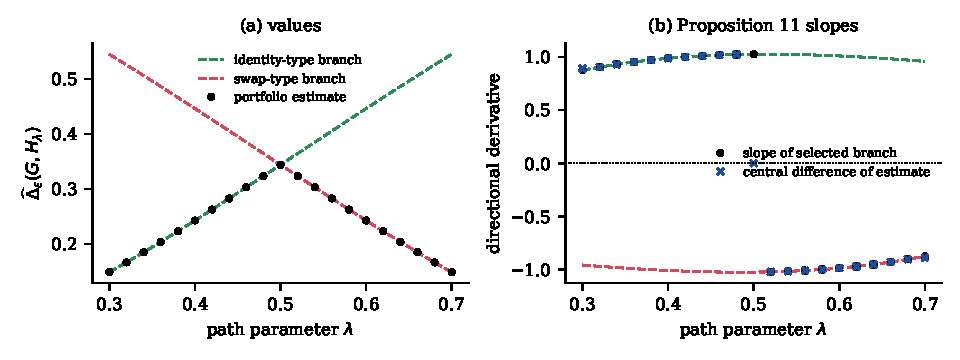
\includegraphics[width=0.85\textwidth]{figures/figS6_branch.pdf}
\caption{A branch crossing. $H_\lambda$ interpolates the geometry of a six-node network and of a copy in which two interchangeable nodes exchange their relations. (a) Values of the two stationary branches (followed by warm starts) and the portfolio estimate (identity, product and attribute starts and six random starts). (b) Directional derivatives along the path from Proposition~11 for each branch, and central differences of the portfolio estimate; at $\lambda=1/2$ the one-sided slopes are $+1.03$ and $-1.03$.}\label{fig:branch}
\end{figure}

\subsection{Additional empirical results}

\begin{table}[h]
\caption{Most influential economies for the anomaly score: total corridor influence $S_i$ on the log-cost scale, imbalance $B_i$, semi-elasticities with respect to log LSCI and log TEU, and mass $\mu_i$.}\label{tab:sensnodes}
\centering\footnotesize
\begin{tabular}{rlrrrrr}
\toprule
Year & economy & $S_i\times10^{3}$ & $B_i$ & $\partial a/\partial\log\mathrm{LSCI}_i$ & $\partial a/\partial\log\mathrm{TEU}_i$ & $\mu_i$\\
\midrule
2016 & China, Hong Kong SAR & 20.8 & $+0.00$ & $1.3\times10^{-3}$ & $4.6\times10^{-3}$ & 0.027\\
 & China & 15.2 & $+0.32$ & $-9.5\times10^{-3}$ & $-2.5\times10^{-4}$ & 0.087\\
 & Singapore & 13.4 & $-0.06$ & $-1.6\times10^{-3}$ & $2.4\times10^{-3}$ & 0.034\\
 & Japan & 9.4 & $+0.27$ & $1.1\times10^{-3}$ & $9.1\times10^{-4}$ & 0.029\\
 & Philippines & 8.9 & $+0.23$ & $1.6\times10^{-4}$ & $1.9\times10^{-3}$ & 0.017\\
 & Malaysia & 8.9 & $+0.05$ & $5.5\times10^{-4}$ & $7\times10^{-5}$ & 0.030\\
\addlinespace
2020 & China, Hong Kong SAR & 11.4 & $+0.16$ & $-1.5\times10^{-3}$ & $3.4\times10^{-3}$ & 0.026\\
 & Singapore & 6.6 & $+0.26$ & $4.0\times10^{-4}$ & $1.6\times10^{-3}$ & 0.037\\
 & China & 6.3 & $-0.12$ & $2.9\times10^{-3}$ & $2.1\times10^{-3}$ & 0.095\\
 & Panama & 5.7 & $-0.06$ & $1.8\times10^{-4}$ & $2.1\times10^{-3}$ & 0.017\\
 & Malta & 5.6 & $+0.53$ & $-1.3\times10^{-3}$ & $2.7\times10^{-3}$ & 0.010\\
 & United Arab Emirates & 5.6 & $-0.48$ & $-8.5\times10^{-4}$ & $1.0\times10^{-3}$ & 0.027\\
\addlinespace
2021 & China, Hong Kong SAR & 15.9 & $+0.06$ & $-1.2\times10^{-3}$ & $4.2\times10^{-3}$ & 0.026\\
 & China & 15.3 & $+0.30$ & $1.4\times10^{-2}$ & $3.7\times10^{-3}$ & 0.098\\
 & Japan & 8.6 & $+0.10$ & $-1.2\times10^{-3}$ & $1.7\times10^{-3}$ & 0.029\\
 & Singapore & 8.2 & $+0.14$ & $1.1\times10^{-3}$ & $2.2\times10^{-3}$ & 0.038\\
 & Philippines & 7.5 & $+0.49$ & $-2.0\times10^{-3}$ & $2.3\times10^{-3}$ & 0.018\\
 & Germany & 6.7 & $-0.23$ & $-1.9\times10^{-3}$ & $1.1\times10^{-3}$ & 0.024\\
\bottomrule
\end{tabular}
\end{table}

\begin{table}[h]
\caption{Corridors with the largest semi-elasticity $\partial a(t)/\partial\log\mathrm{cost}_{ik}$, with the semi-elasticity of the reverse corridor.}\label{tab:senscorr}
\centering\footnotesize
\begin{tabular}{rllrrr}
\toprule
Year & origin & destination & cost (USD/kg) & semi-elasticity & reverse\\
\midrule
2020 & Malta & China & 5.24 & $1.9\times10^{-3}$ & $2.2\times10^{-5}$\\
 & China, Hong Kong SAR & United Arab Emirates & 3.24 & $-1.8\times10^{-3}$ & $6.2\times10^{-4}$\\
 & Morocco & Ecuador & 3.72 & $7.3\times10^{-4}$ & $9.2\times10^{-7}$\\
 & Dominican Republic & Egypt & 13.49 & $6.8\times10^{-4}$ & $-1.5\times10^{-6}$\\
 & Colombia & Egypt & 2.41 & $6.5\times10^{-4}$ & $-1.6\times10^{-6}$\\
 & United Arab Emirates & China, Hong Kong SAR & 4.23 & $6.2\times10^{-4}$ & $-1.8\times10^{-3}$\\
 & Singapore & Morocco & 1.16 & $5.6\times10^{-4}$ & $2.1\times10^{-6}$\\
 & Ghana & China, Hong Kong SAR & 7.50 & $5.4\times10^{-4}$ & $-8.6\times10^{-6}$\\
\addlinespace
2021 & Malta & China & 6.34 & $1.7\times10^{-3}$ & $2.7\times10^{-5}$\\
 & China, Hong Kong SAR & United Arab Emirates & 3.46 & $-1.5\times10^{-3}$ & $2.5\times10^{-4}$\\
 & Jamaica & China, Hong Kong SAR & 10.51 & $9.8\times10^{-4}$ & $2.2\times10^{-5}$\\
 & Malta & China, Hong Kong SAR & 20.72 & $9.3\times10^{-4}$ & $9.4\times10^{-7}$\\
 & Morocco & China, Hong Kong SAR & 3.01 & $8.8\times10^{-4}$ & $-4.7\times10^{-5}$\\
\bottomrule
\end{tabular}
\end{table}

\begin{table}[h]
\caption{First-order predictions of the gradient strategy and re-solved changes. (i) $\Delta(G_{2020},G_{2021})$, with the cross-term change, its first-order prediction and the frozen-coupling remainder $R_P$ of Proposition~14(a). (ii) $a(2020)$. (iii) $\hat\tau(\mathrm{EAP},\mathrm{SSEA})$. Portfolio and branch-following values agreed in every case.}\label{tab:sensacc}
\centering\footnotesize
\begin{tabular}{lrrrrrrr}
\toprule
 & $B$ & predicted & realized & ratio & cross-term change & cross-term prediction & $R_P$\\
\midrule
(i) & 1 & $-1.54\times10^{-3}$ & $-1.34\times10^{-3}$ & 0.87 & $-1.34\times10^{-3}$ & $-1.49\times10^{-3}$ & $2.0\times10^{-4}$\\
 & 4 & $-4.20\times10^{-3}$ & $-2.89\times10^{-3}$ & 0.69 & $-2.96\times10^{-3}$ & $-4.03\times10^{-3}$ & $1.2\times10^{-3}$\\
 & 16 & $-1.10\times10^{-2}$ & $-7.45\times10^{-3}$ & 0.68 & $-7.60\times10^{-3}$ & $-1.04\times10^{-2}$ & $3.2\times10^{-3}$\\
 & 64 & $-2.39\times10^{-2}$ & $-1.59\times10^{-2}$ & 0.66 & $-1.62\times10^{-2}$ & $-2.28\times10^{-2}$ & $7.7\times10^{-3}$\\
 & 128 & $-3.36\times10^{-2}$ & $-2.16\times10^{-2}$ & 0.64 & $-2.23\times10^{-2}$ & $-3.20\times10^{-2}$ & $1.1\times10^{-2}$\\
\addlinespace
(ii) & 8 & $5.3\times10^{-3}$ & $6.6\times10^{-3}$ & 1.25 & & & \\
 & 32 & $1.17\times10^{-2}$ & $1.47\times10^{-2}$ & 1.26 & & & \\
 & 128 & $2.20\times10^{-2}$ & $3.05\times10^{-2}$ & 1.39 & & & \\
 & 512 & $3.30\times10^{-2}$ & $5.03\times10^{-2}$ & 1.52 & & & \\
 & 2048 & $3.95\times10^{-2}$ & $6.30\times10^{-2}$ & 1.59 & & & \\
\addlinespace
(iii) & 0.5 & $-0.014$ & $-0.027$ & 1.87 & & & \\
 & 2 & $-0.043$ & $-0.064$ & 1.50 & & & \\
 & 8 & $-0.101$ & $-0.136$ & 1.35 & & & \\
 & 16 & $-0.146$ & $-0.186$ & 1.27 & & & \\
\bottomrule
\end{tabular}
\end{table}

\begin{table}[h]
\caption{Delta-method and Monte Carlo standard deviations of the anomaly scores and of two margins under independent multiplicative cost errors with log-scale standard deviation $\sigma_m$ (12 replications per level, all problems re-solved). Shift: Monte Carlo mean minus baseline. Rank: mean Monte Carlo rank.}\label{tab:sensunc}
\centering\footnotesize
\begin{tabular}{lrrrrrrrr}
\toprule
 & \multicolumn{4}{c}{$\sigma_m=0.10$} & \multicolumn{4}{c}{$\sigma_m=0.25$}\\
\cmidrule(lr){2-5}\cmidrule(lr){6-9}
 & delta s.d. & MC s.d. & shift & rank & delta s.d. & MC s.d. & shift & rank\\
\midrule
$a(2016)$ & 0.68 & 0.50 & 2.43 & 1.00 & 1.71 & 1.43 & 14.43 & 1.00\\
$a(2017)$ & 0.51 & 0.39 & 2.41 & 4.92 & 1.27 & 1.25 & 13.53 & 4.58\\
$a(2018)$ & 0.48 & 0.39 & 2.31 & 6.00 & 1.19 & 1.02 & 13.03 & 6.00\\
$a(2019)$ & 0.48 & 0.44 & 2.34 & 3.00 & 1.20 & 1.22 & 13.16 & 3.08\\
$a(2020)$ & 0.50 & 0.39 & 2.35 & 4.08 & 1.25 & 1.28 & 13.41 & 4.33\\
$a(2021)$ & 0.59 & 0.54 & 2.38 & 2.00 & 1.47 & 1.29 & 14.59 & 2.00\\
\addlinespace
$a(2016)-a(2020)$ & 0.66 & 0.51 & 0.09 & -- & 1.64 & 2.30 & 1.01 & --\\
$a(2021)-a(2020)$ & 0.60 & 0.52 & 0.03 & -- & 1.51 & 1.73 & 1.17 & --\\
\bottomrule
\multicolumn{9}{l}{\scriptsize All entries except ranks $\times10^{-3}$.}
\end{tabular}
\end{table}

\begin{figure}[h]
\centering
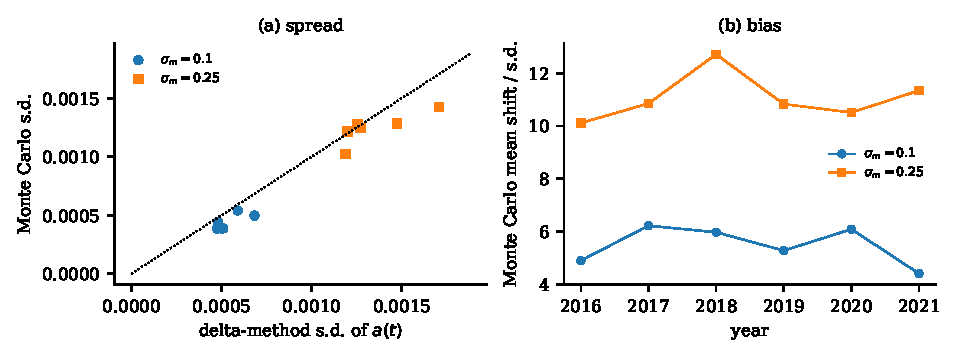
\includegraphics[width=0.85\textwidth]{figures/figS7_uncertainty.pdf}
\caption{(a) Monte Carlo against delta-method standard deviations of the anomaly scores. (b) Monte Carlo mean shift of each score in units of its Monte Carlo standard deviation.}\label{fig:sensunc}
\end{figure}

Dropping 5\% of the observed pairs at random in every year (four draws) left the anomaly ranking unchanged in every draw. The Spearman correlation of the corridor sensitivities with the baseline was at least 0.93 and that of the economy influence at least 0.975; at least 87\% of the hundred most influential corridors and 90\% of the ten most influential economies were retained in every year.
